\fakesection{Function Estimation and Time Series Prediction}{\hfill\small\texttt{/src/session\_2/.m}}

\fakesubsection{Support vector machine for function estimation}{}

Since the use of a linear kernel for function estimation is equivalent to linear regression one can expect it to perform better than any other kernel when the function to be estimated happens to be linear. Non-linear datasets are more challenging such that other kernels which enable the SVM to model non-linear functions can be used instead. The examples given in figure \ref{functionestimation} shouldn't be taken too seriously - there's no test set and some of the results such as that of the RBF kernel ($\sigma^2=0.1$) and the exponential kernel are likely to overfit.

\begin{figure}[h]
\centering
\subfloat[Linear kernel.]{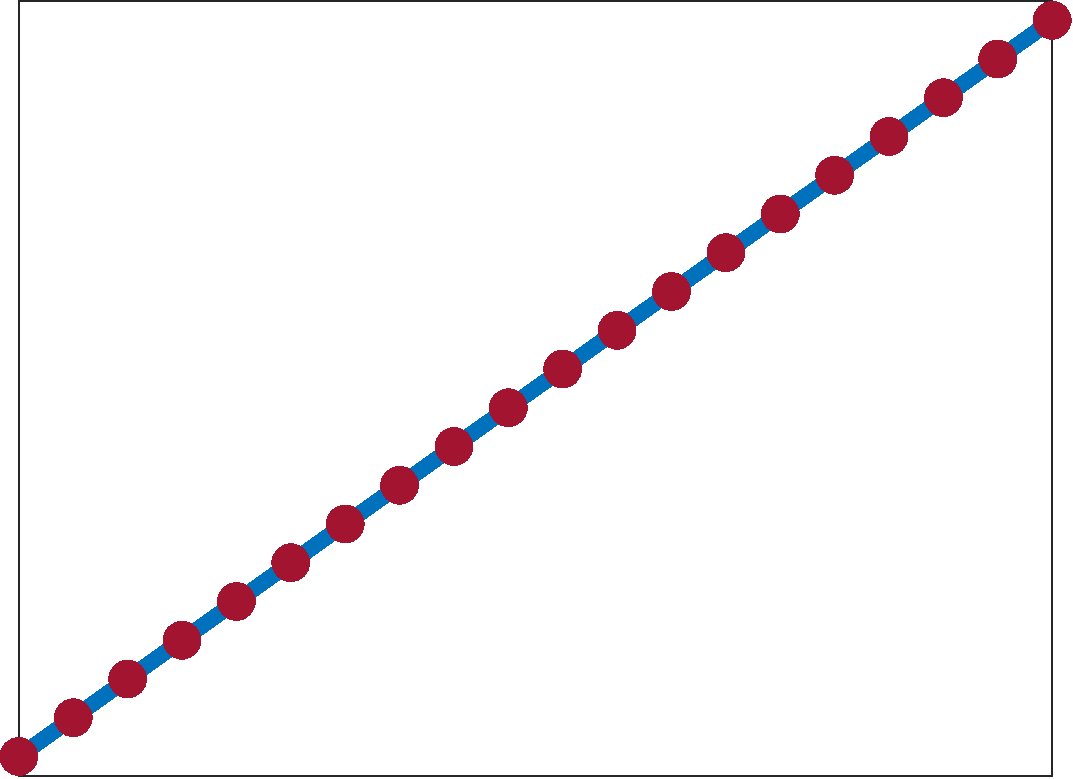
\includegraphics[width=0.16\textwidth]{../src/figures/estimation/gui_linear}}\qquad
\subfloat[Polynomial kernel, $\delta=3$.]{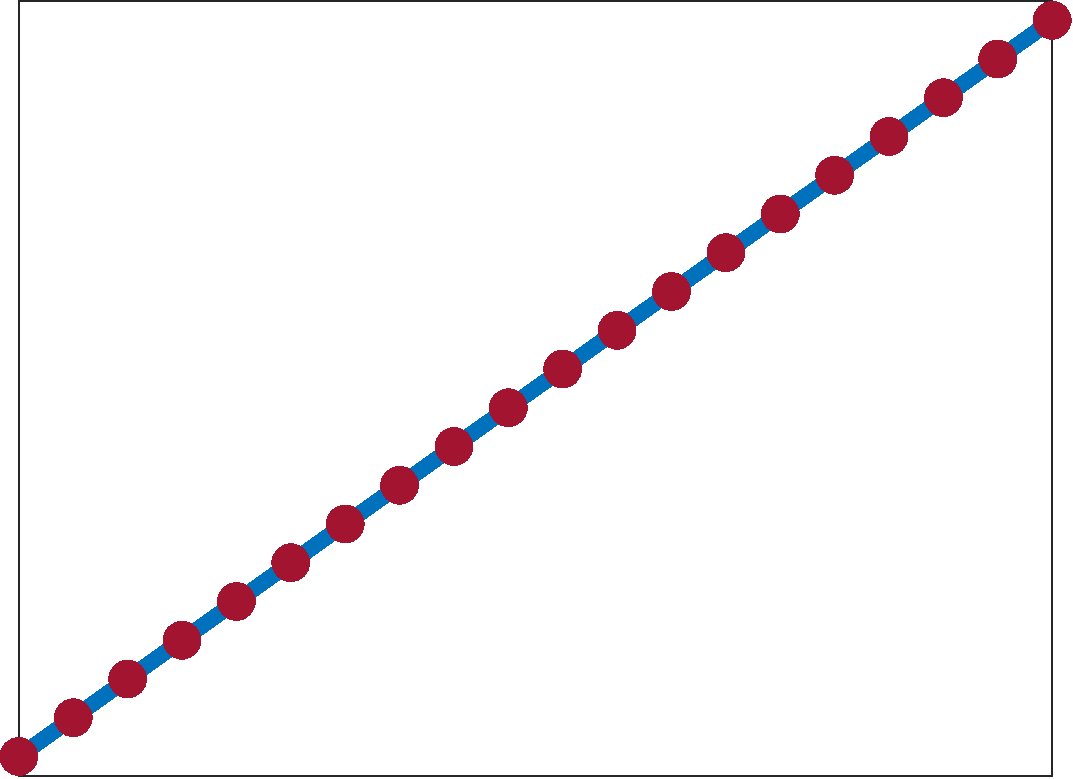
\includegraphics[width=0.16\textwidth]{../src/figures/estimation/gui_polynomial}}\qquad
\subfloat[RBF kernel, $\sigma^2=1$.]{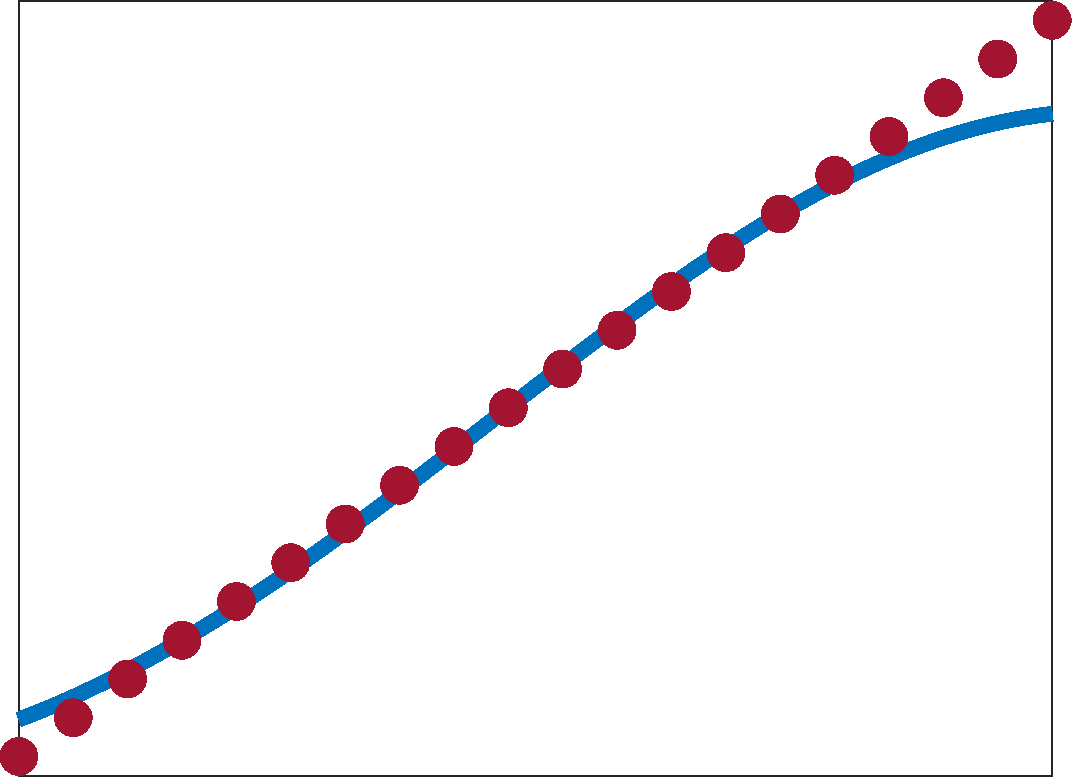
\includegraphics[width=0.16\textwidth]{../src/figures/estimation/gui_rbf}}\qquad
\subfloat[Trigonometric kernel, degree 1.]{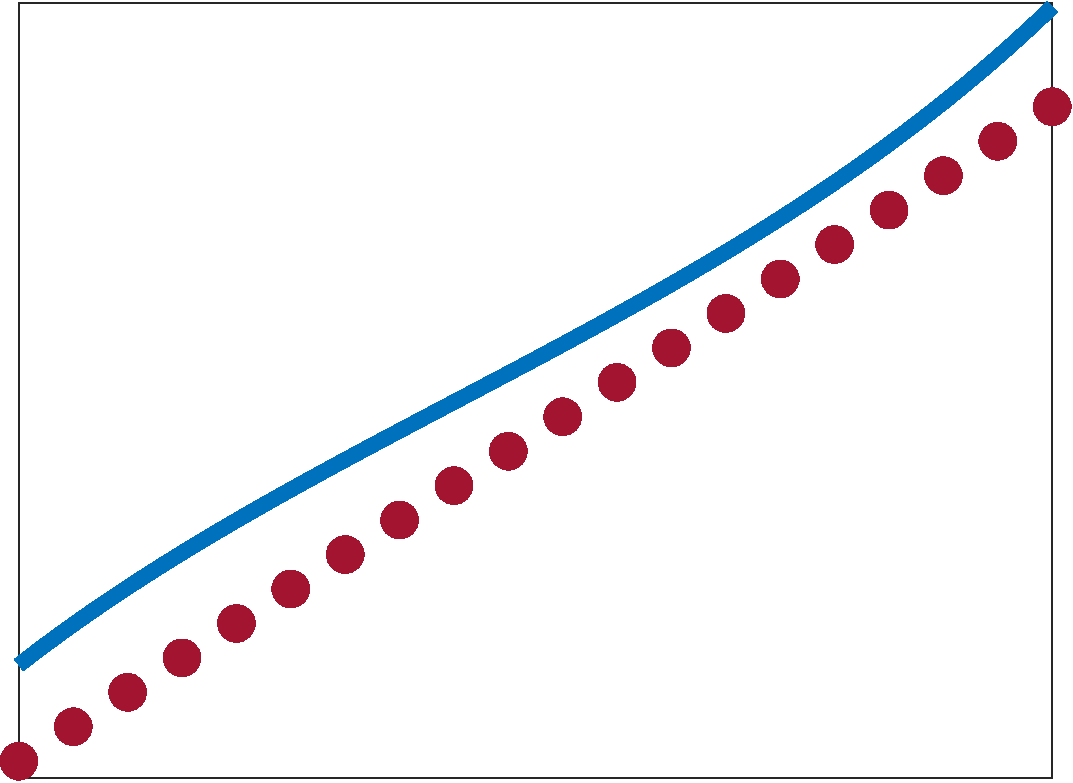
\includegraphics[width=0.16\textwidth]{../src/figures/estimation/gui_trigonometric}}\qquad
\subfloat[Exponential kernel, $\sigma^2=1$.]{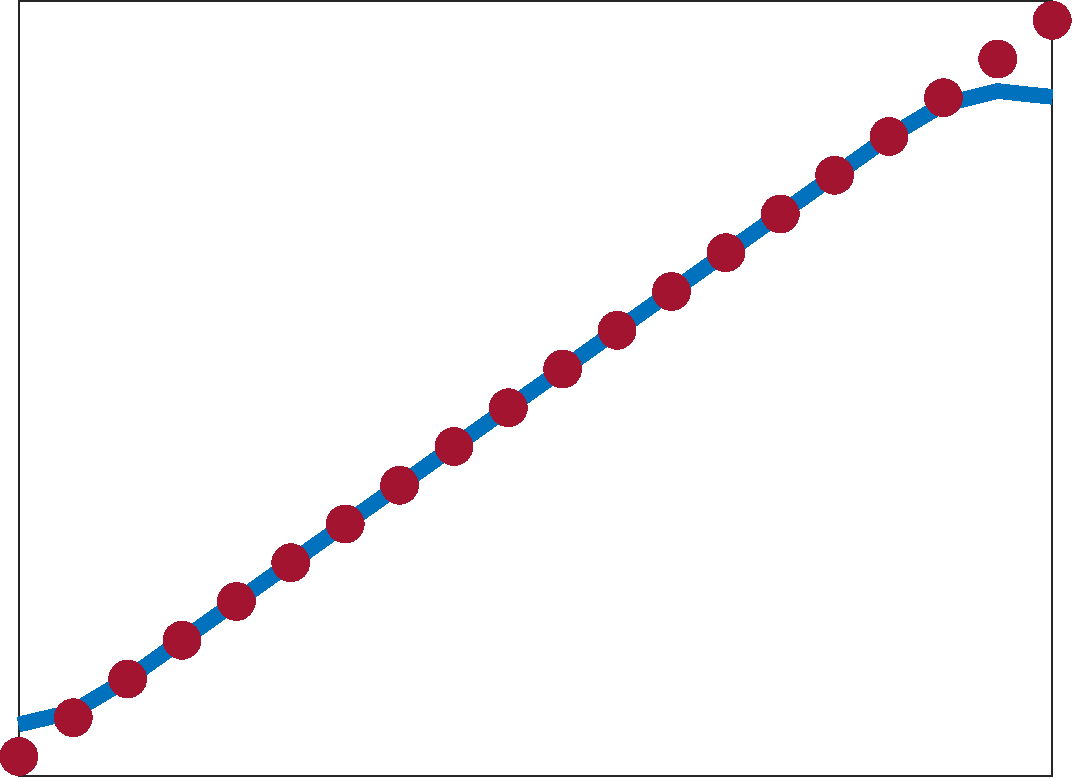
\includegraphics[width=0.16\textwidth]{../src/figures/estimation/gui_exponential}}\qquad
\\
\subfloat[Linear kernel.]{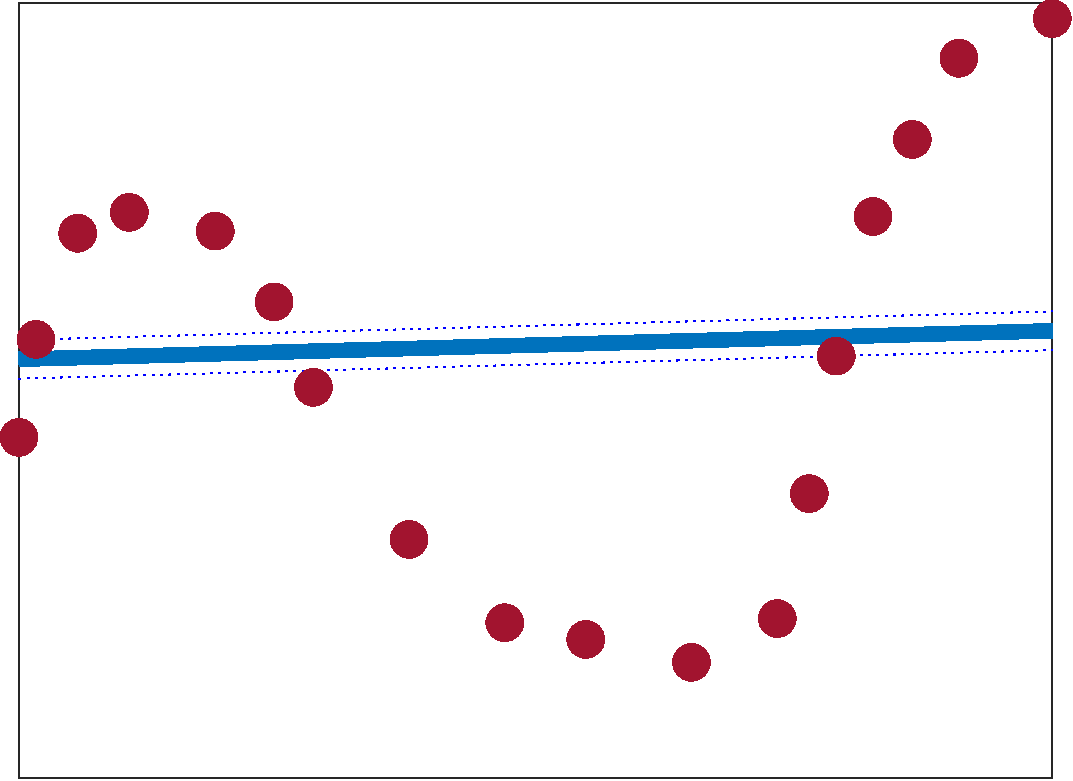
\includegraphics[width=0.16\textwidth]{../src/figures/estimation/gui_nonlinear_linear}}\qquad
\subfloat[Polynomial kernel, $\delta=3$.]{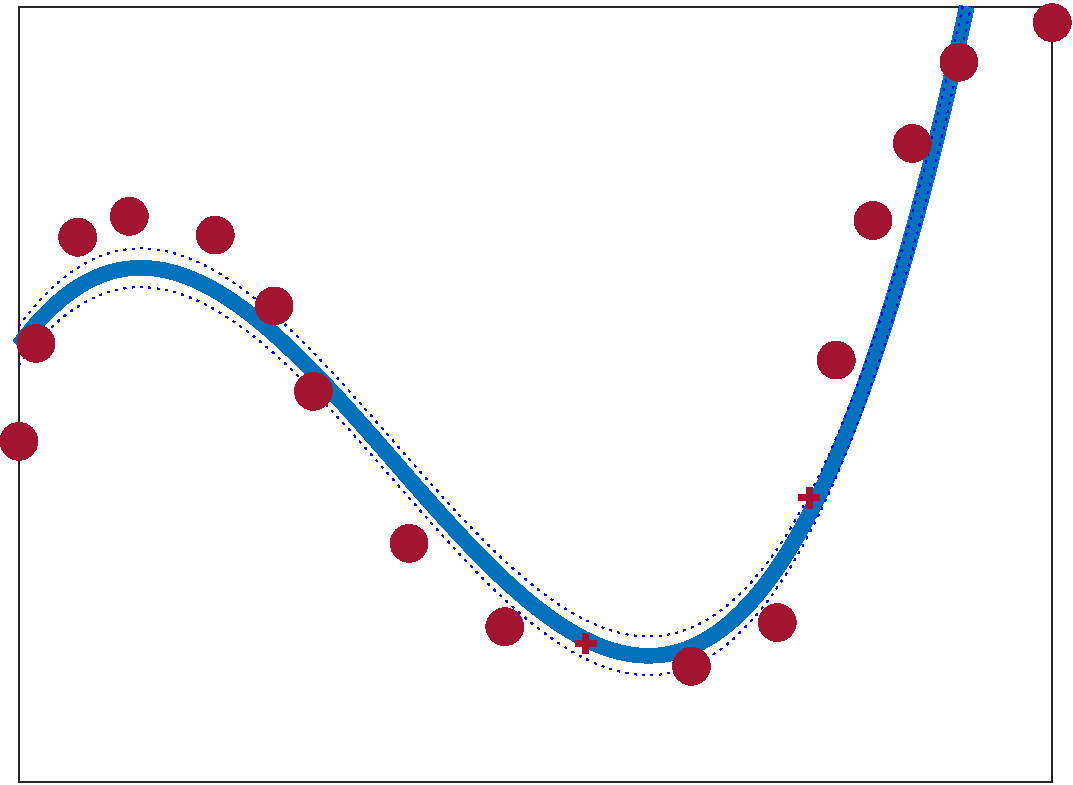
\includegraphics[width=0.16\textwidth]{../src/figures/estimation/gui_nonlinear_polynomial}}\qquad
\subfloat[RBF kernel, $\sigma^2=0.1$.]{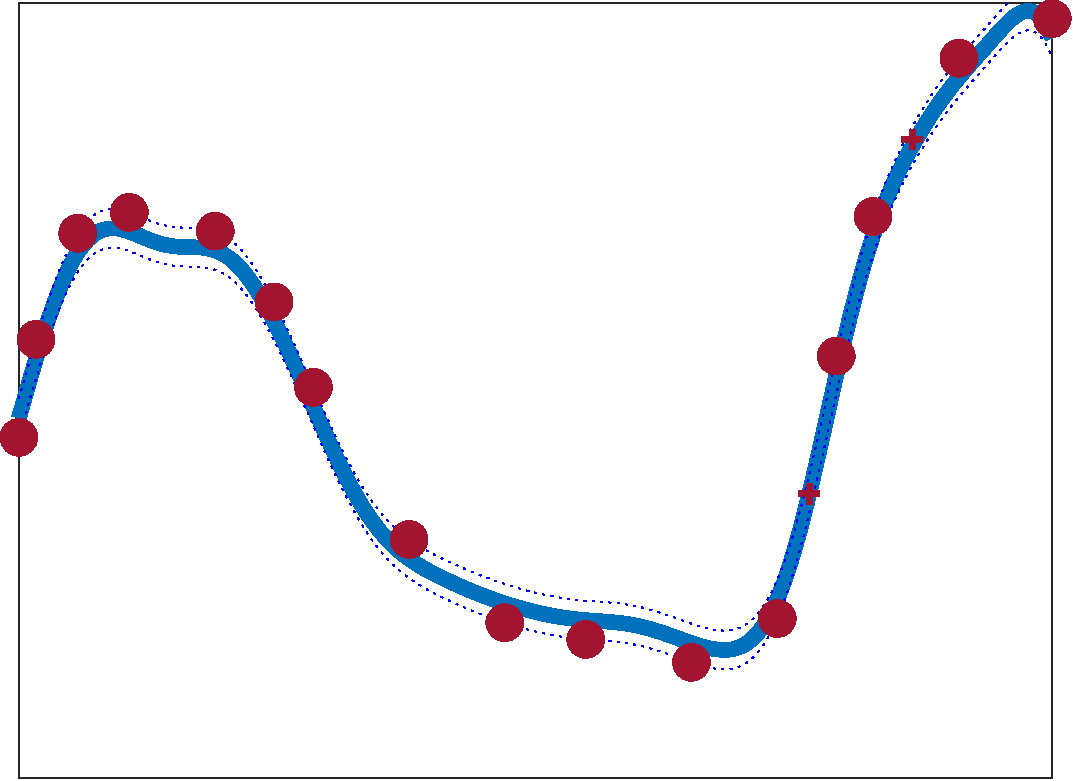
\includegraphics[width=0.16\textwidth]{../src/figures/estimation/gui_nonlinear_rbf}}\qquad
\subfloat[Linear b-spline kernel, degree 5.]{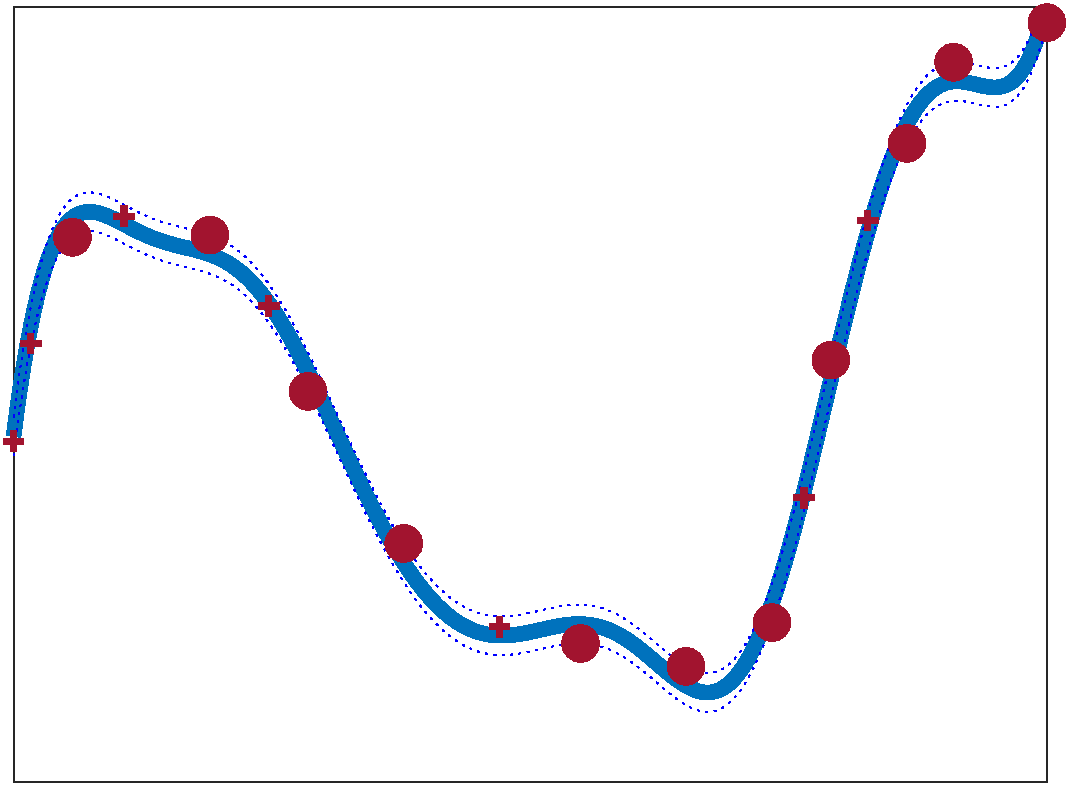
\includegraphics[width=0.16\textwidth]{../src/figures/estimation/gui_nonlinear_bspline}}\qquad
\subfloat[Exponential kernel, $\sigma^2=0.1$.]{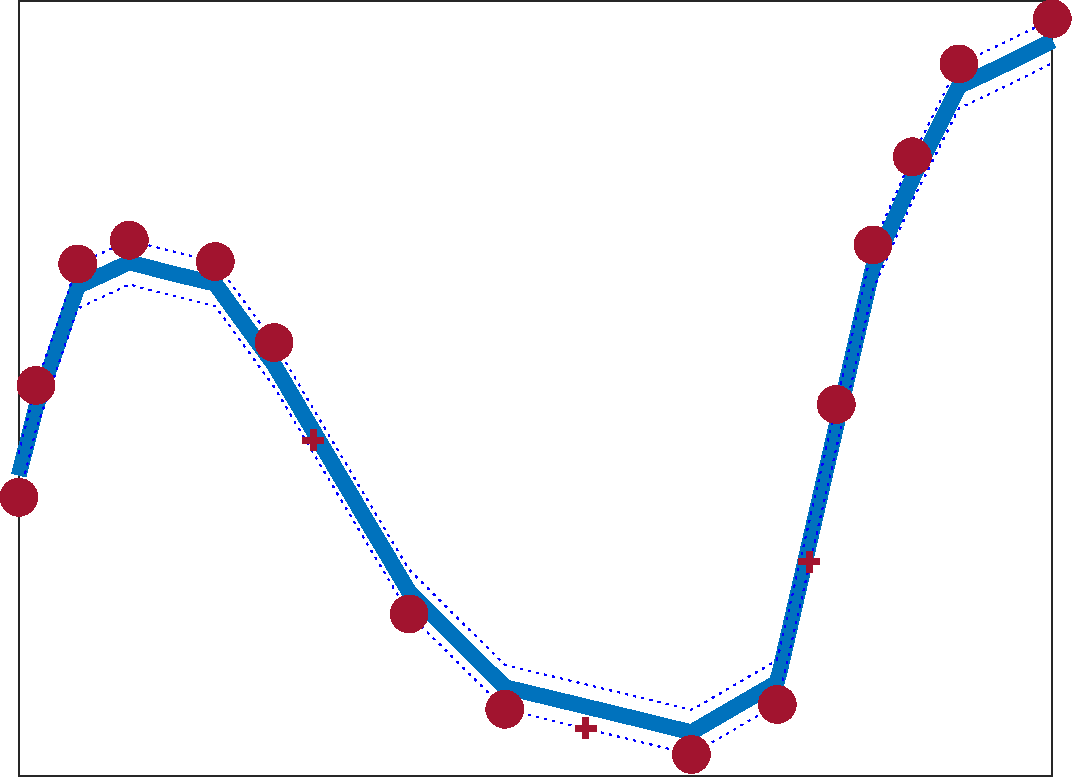
\includegraphics[width=0.16\textwidth]{../src/figures/estimation/gui_nonlinear_exponential}}\qquad
\caption{Visualisation of the results of experiments with various kernels and parameters for two different datasets. In the first row $\epsilon=0$ and \texttt{bound} = 10, in the second one $\epsilon=1$ and \texttt{bound} = 1000.}
\label{functionestimation}
\end{figure}

\fakesubsection{A simple example: the sinc function}{}

\begin{figure}[h]
\centering
\subfloat[$\gamma=10,\sigma=0.01$]{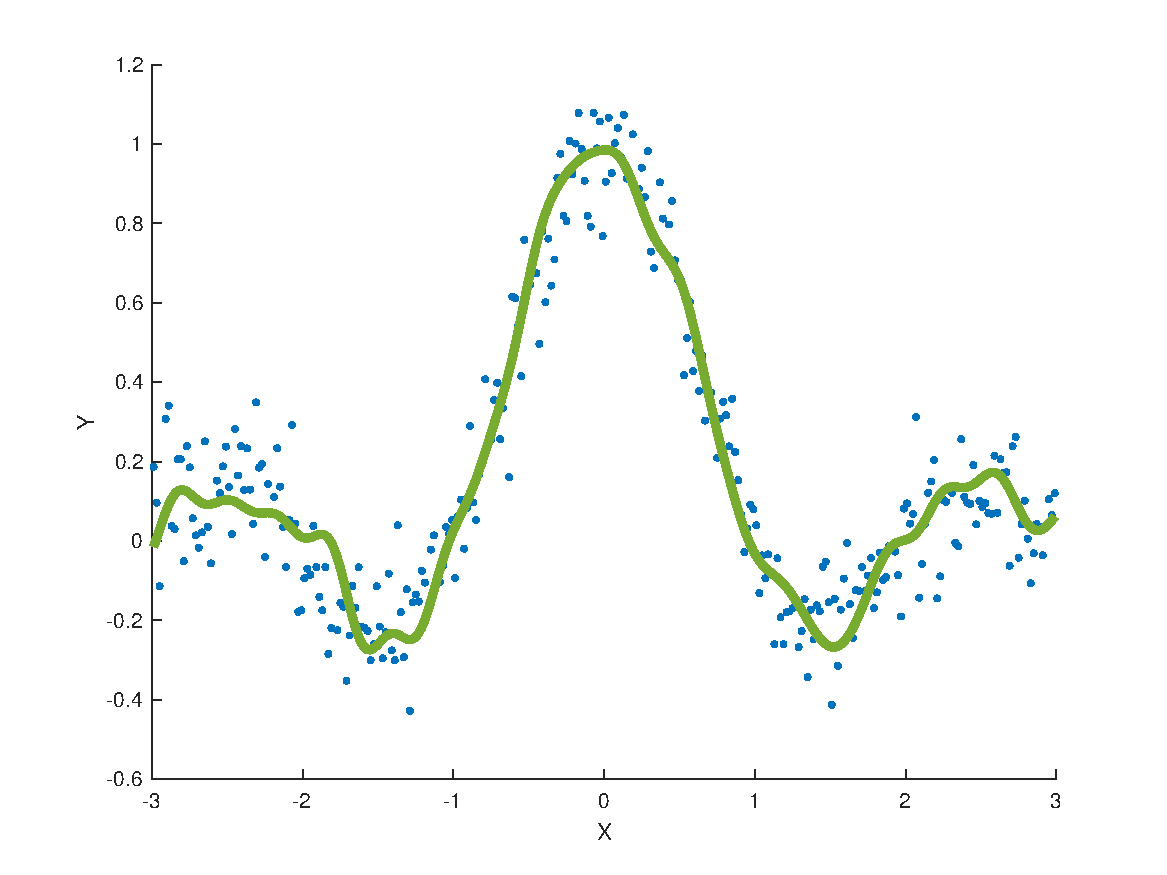
\includegraphics[width=0.3\textwidth]{../src/figures/estimation/regression_1}}\qquad
\subfloat[$\gamma=10,\sigma=1$]{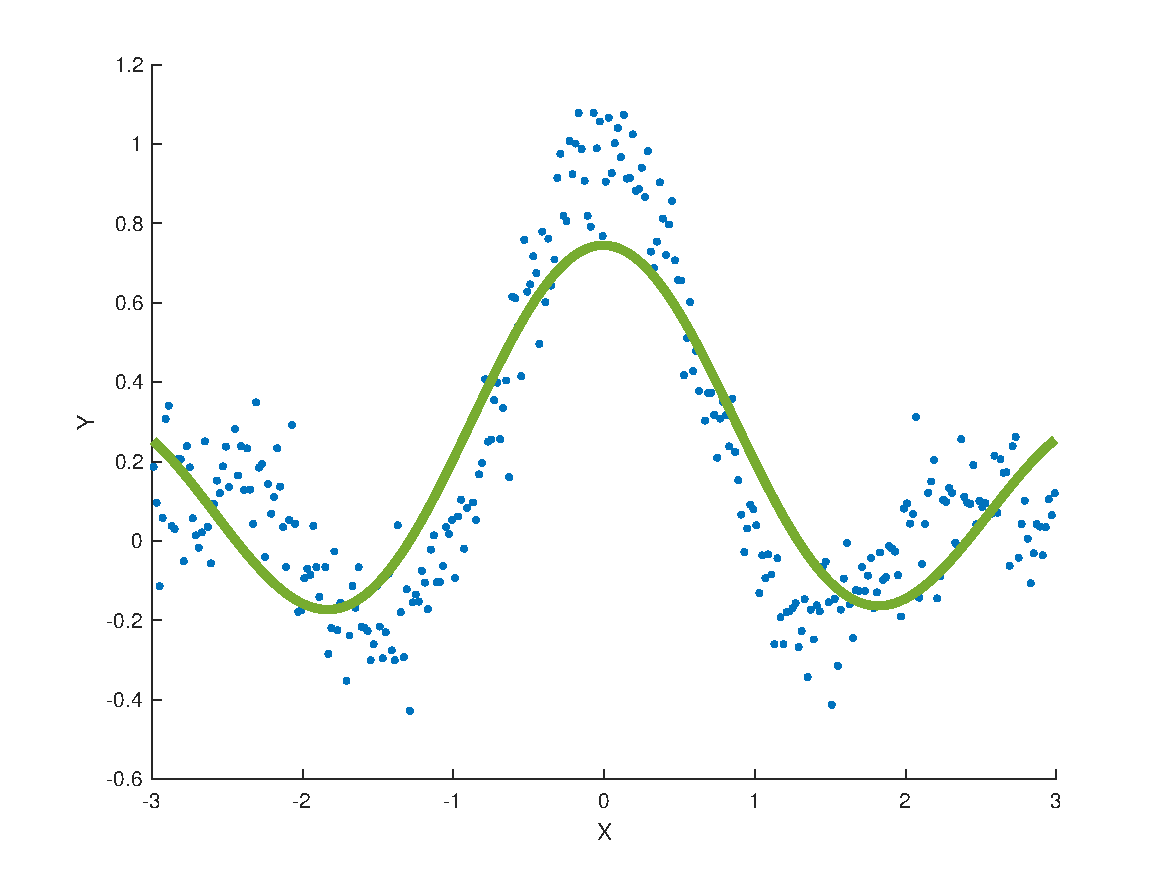
\includegraphics[width=0.3\textwidth]{../src/figures/estimation/regression_2}}\qquad
\subfloat[$\gamma=10,\sigma=100$]{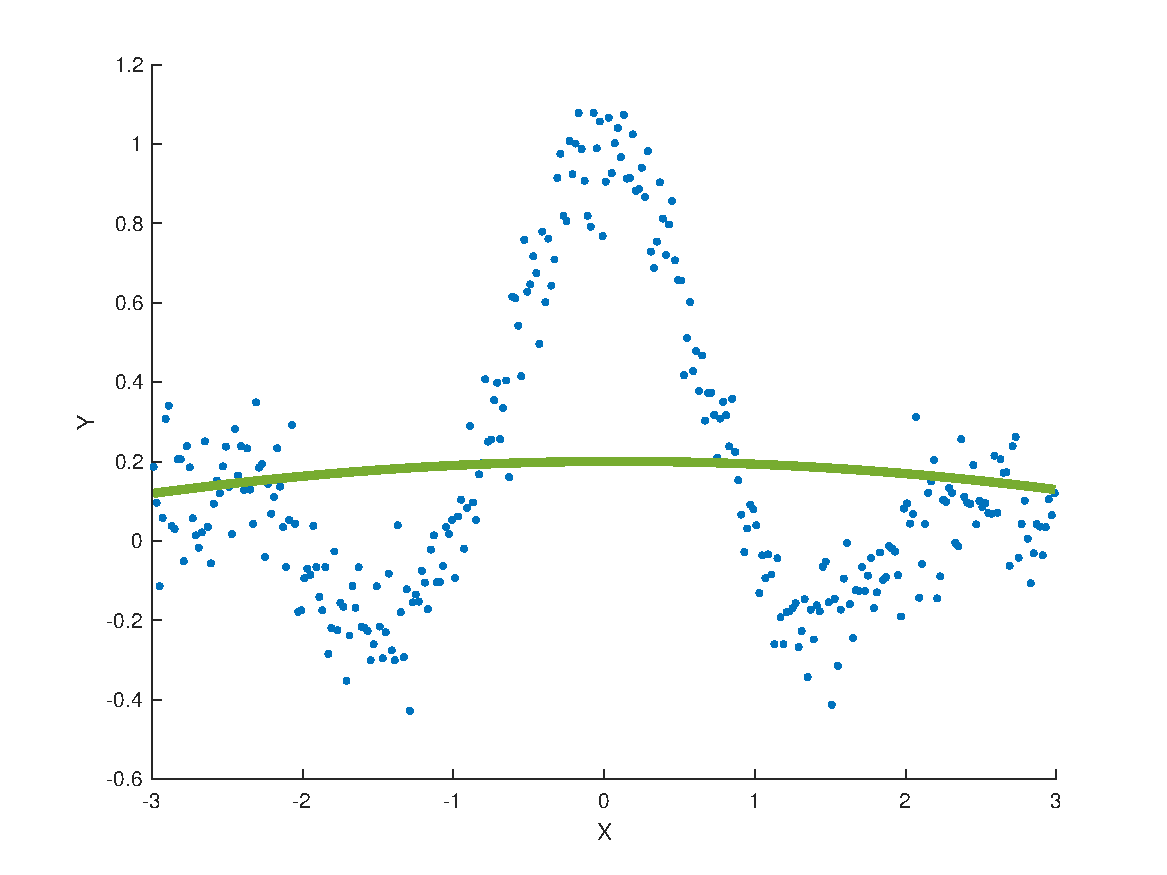
\includegraphics[width=0.3\textwidth]{../src/figures/estimation/regression_3}}\qquad
\\
\subfloat[$\gamma=10^3,\sigma=0.01$]{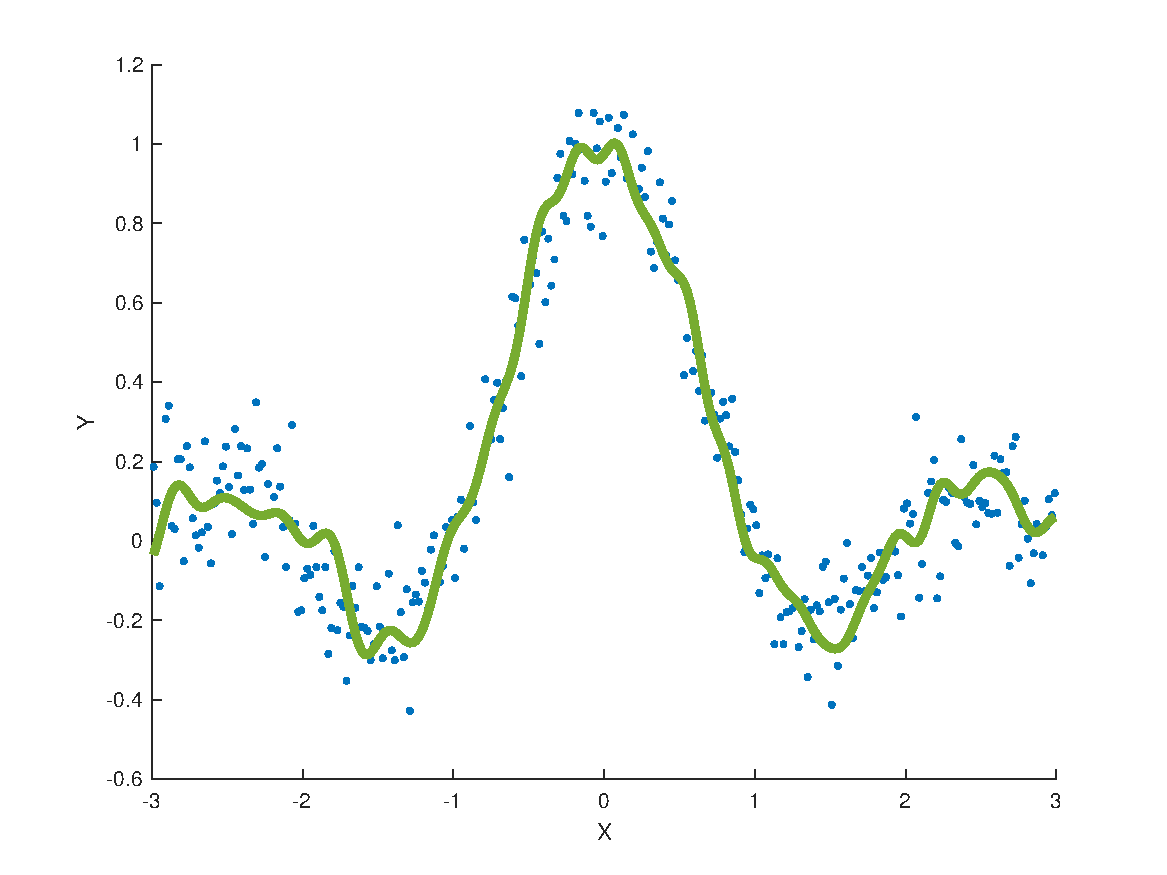
\includegraphics[width=0.3\textwidth]{../src/figures/estimation/regression_4}}\qquad
\subfloat[$\gamma=10^3,\sigma=1$]{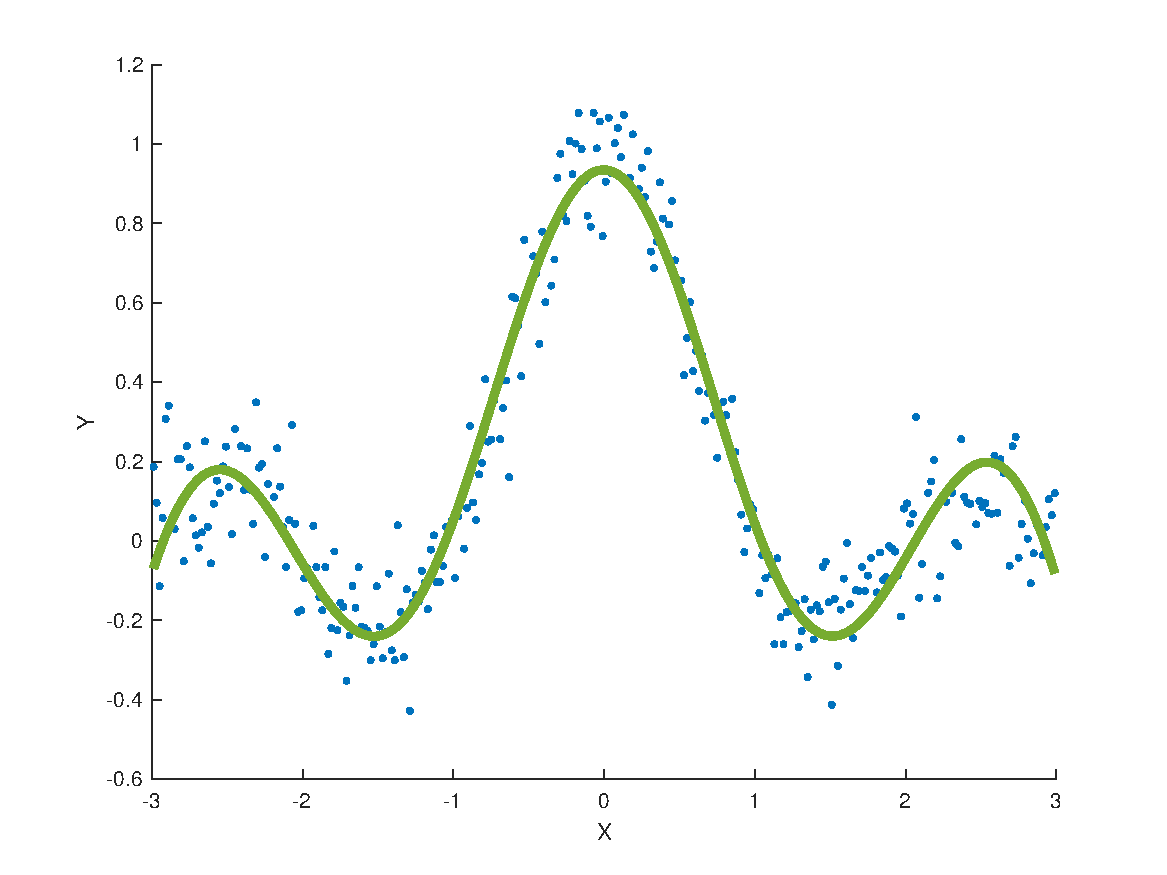
\includegraphics[width=0.3\textwidth]{../src/figures/estimation/regression_5}}\qquad
\subfloat[$\gamma=10^3,\sigma=100$]{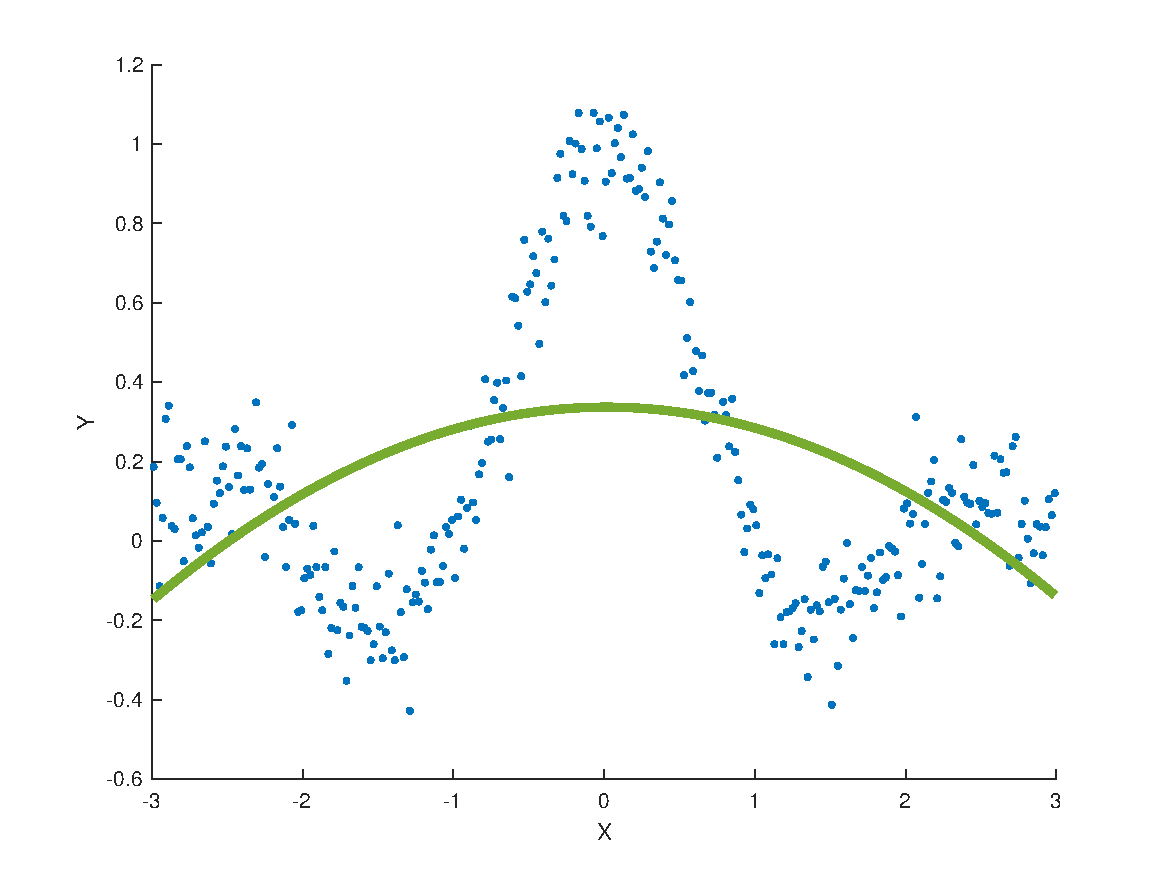
\includegraphics[width=0.3\textwidth]{../src/figures/estimation/regression_6}}\qquad
\\
\subfloat[$\gamma=10^6,\sigma=0.01$]{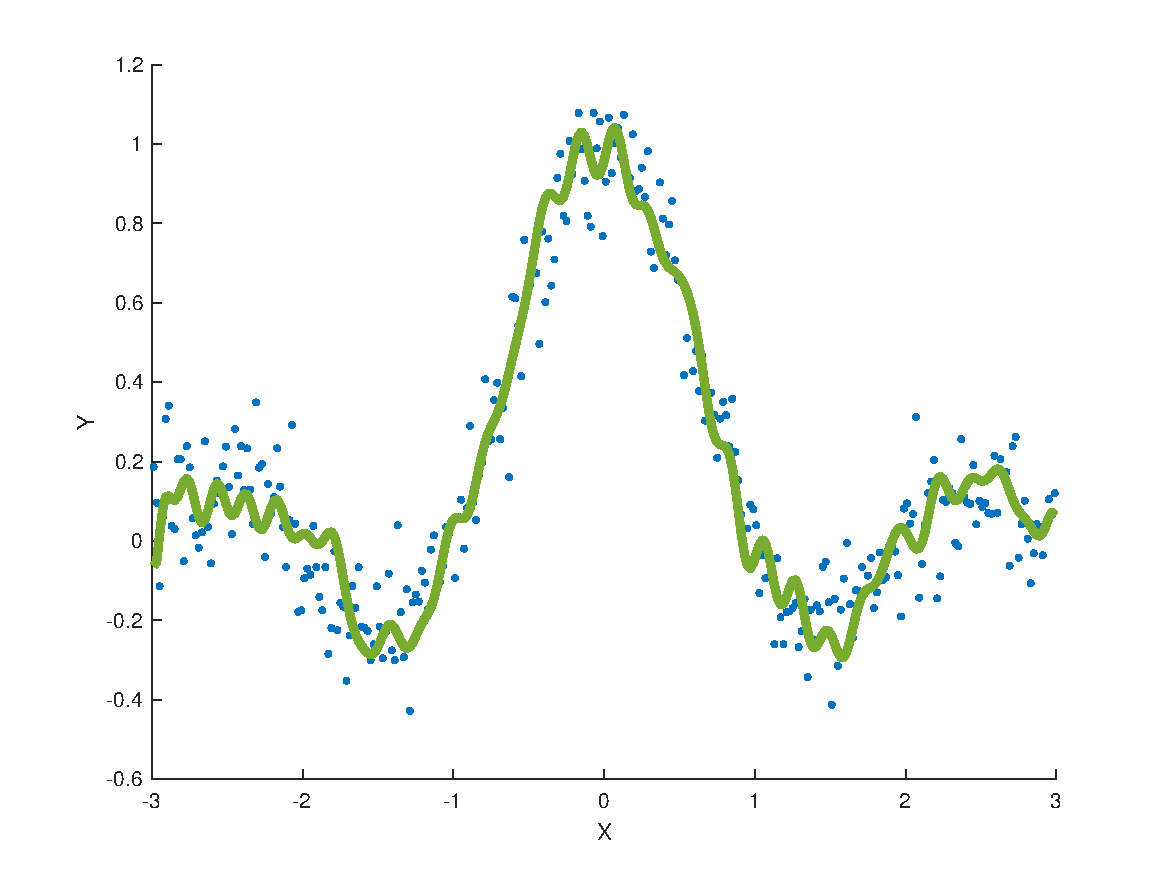
\includegraphics[width=0.3\textwidth]{../src/figures/estimation/regression_7}}\qquad
\subfloat[$\gamma=10^6,\sigma=1$]{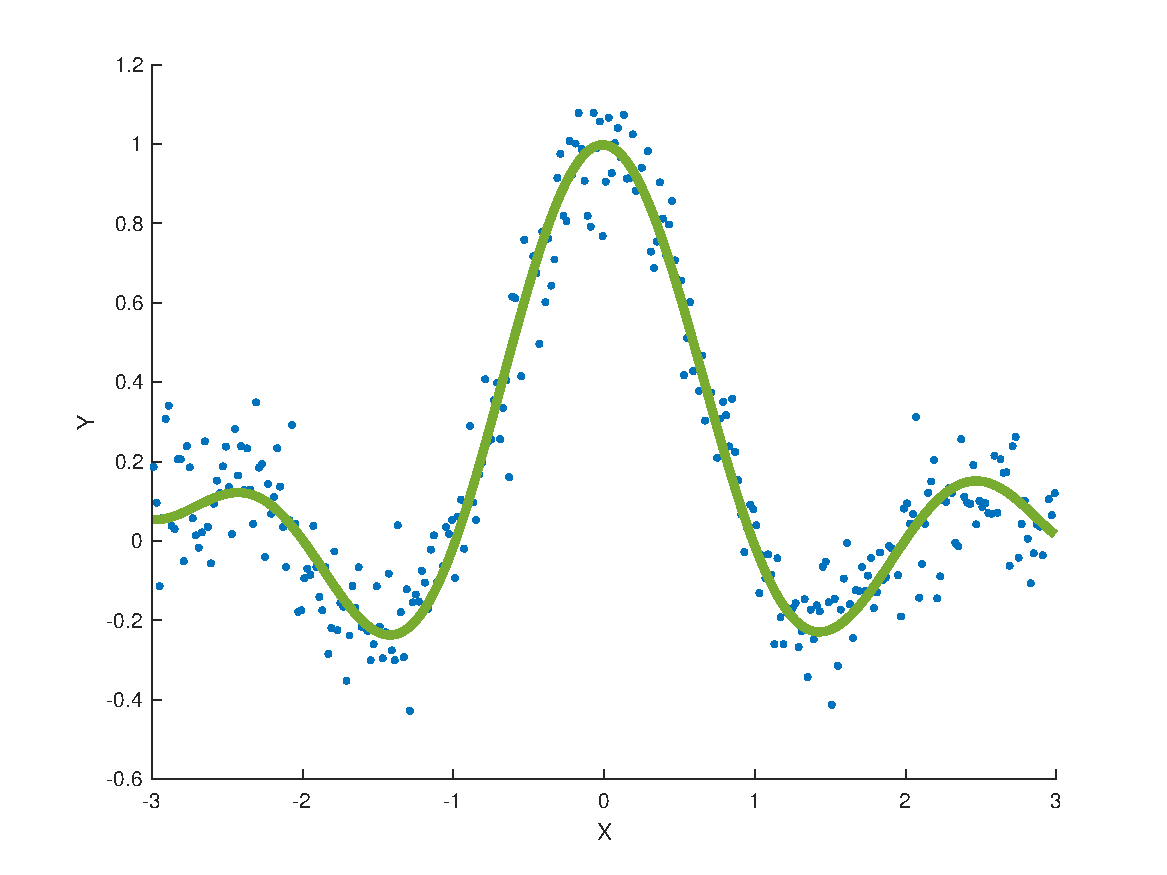
\includegraphics[width=0.3\textwidth]{../src/figures/estimation/regression_8}}\qquad
\subfloat[$\gamma=10^6,\sigma=100$]{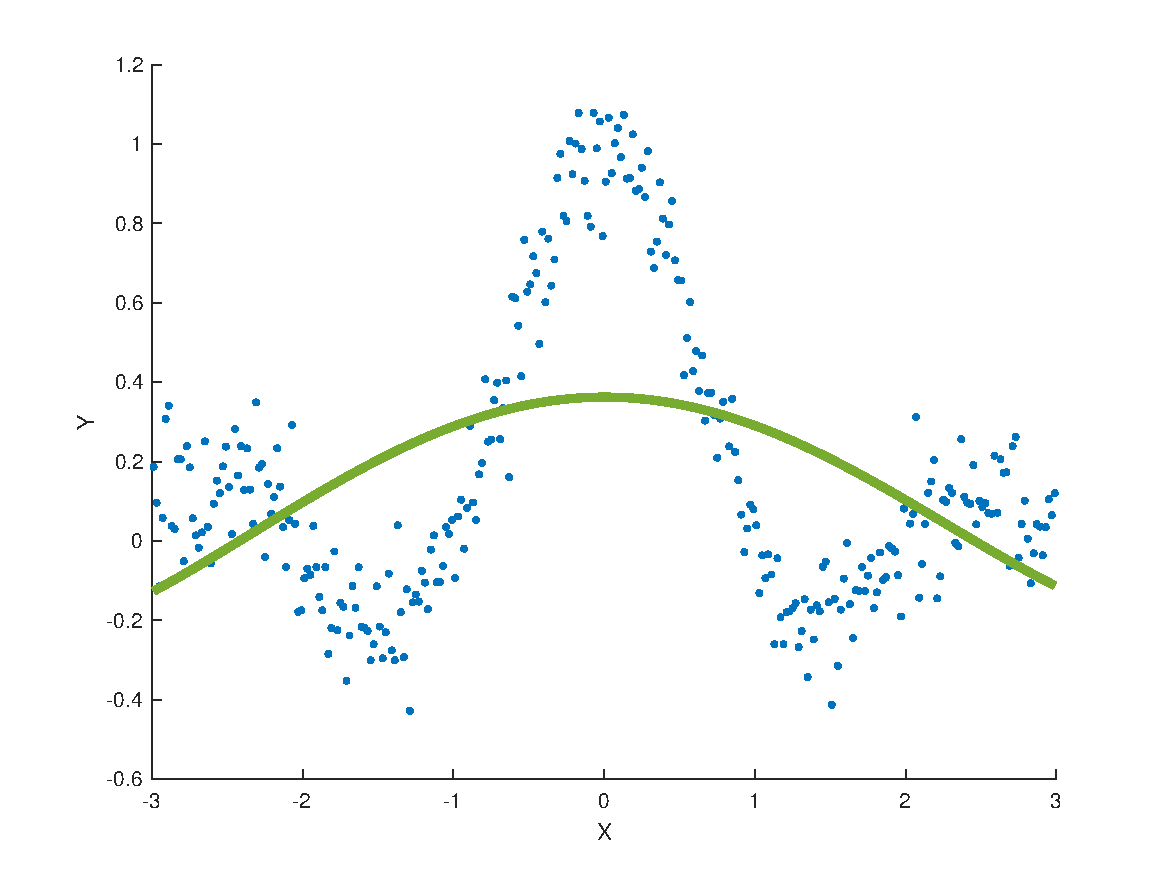
\includegraphics[width=0.3\textwidth]{../src/figures/estimation/regression_9}}\qquad
\caption{Function estimation experiments with the \texttt{sinc} function. Noisy samples are fed to an LS-SVM. The green line is the estimated model, the blue dots represent the test data.}
\label{sincestimate}
\end{figure}

\fakesubsection{Automatic Relevance Determination}{}



\fakesubsection{Robust regression}{}

By applying cross-validation on any subset of the input features one can consider the most promising subset as having the relevant features.

\fakesubsection{Introduction: time series prediction}{}


\fakesubsection{Logmap dataset}{}


\fakesubsection{Santa Fe dataset}{}



